%\title{LaTeX Portrait Poster Template}
%%%%%%%%%%%%%%%%%%%%%%%%%%%%%%%%%%%%%%%%%
% a0poster Portrait Poster
% LaTeX Template
% Version 1.0 (22/06/13)
%
% The a0poster class was created by:
% Gerlinde Kettl and Matthias Weiser (tex@kettl.de)
% 
% Adapter by Jens Buysse for Hogeschool Gent
% This template has been downloaded from:
% http://www.LaTeXTemplates.com
%
% License:
% CC BY-NC-SA 3.0 (http://creativecommons.org/licenses/by-nc-sa/3.0/)
%
%%%%%%%%%%%%%%%%%%%%%%%%%%%%%%%%%%%%%%%%%

%----------------------------------------------------------------------------------------
%	PACKAGES AND OTHER DOCUMENT CONFIGURATIONS
%----------------------------------------------------------------------------------------

\documentclass[a0,portrait]{a0poster}

\usepackage{multicol} % This is so we can have multiple columns of text side-by-side
\columnsep=100pt % This is the amount of white space between the columns in the poster
\columnseprule=3pt % This is the thickness of the black line between the columns in the poster

\usepackage[svgnames]{xcolor} % Specify colors by their 'svgnames', for a full list of all colors available see here: http://www.latextemplates.com/svgnames-colors

\usepackage{times} % Use the times font
%\usepackage{palatino} % Uncomment to use the Palatino font

\usepackage{graphicx} % Required for including images
\graphicspath{{figures/}} % Location of the graphics files
\usepackage{booktabs} % Top and bottom rules for table
\usepackage[font=small,labelfont=bf]{caption} % Required for specifying captions to tables and figures
\usepackage{amsfonts, amsmath, amsthm, amssymb} % For math fonts, symbols and environments
\usepackage{wrapfig} % Allows wrapping text around tables and figures
\usepackage[export]{adjustbox}

\begin{document}

%----------------------------------------------------------------------------------------
%	POSTER HEADER 
%----------------------------------------------------------------------------------------

% The header is divided into two boxes:
% The first is 75% wide and houses the title, subtitle, names, university/organization and contact information
% The second is 25% wide and houses a logo for your university/organization or a photo of you
% The widths of these boxes can be easily edited to accommodate your content as you see fit

\begin{minipage}[t]{0.75\linewidth}
\VeryHuge \color{HoGentAccent1} \textbf{Een vergelijkende studie tussen Data Vault 2.0 en het dimensioneel model bij het modelleren van een data warehouse.} \color{Black}\\ % Title
\huge \textbf{Spiesschaert Jorik, Lievens Stijn, Stroobants Jochen}\\[0.5cm] % Author(s)
\huge Hogeschool Gent, Valentin Vaerwyckweg 1, 9000 Gent\\[0.4cm] % University/organization
\Large \texttt{jorik.spiesschaert.y9481@hogent.be} \\
\end{minipage}
%
\begin{minipage}[t]{0.25\linewidth}

\includegraphics[width=13cm,right]{figures/HG-woordmerk.png} 

\end{minipage}

\vspace{1cm} % A bit of extra whitespace between the header and poster content

%----------------------------------------------------------------------------------------

\begin{multicols}{2} % This is how many columns your poster will be broken into, a portrait poster is generally split into 2 columns

%----------------------------------------------------------------------------------------
%	ABSTRACT
%----------------------------------------------------------------------------------------

\color{HoGentAccent1} % Navy color for the abstract

\begin{abstract}
Bij het modelleren van een data warehouse moet rekening gehouden worden met de noden van een organisatie. Afhankelijk van die noden, kan er beslist worden om een bepaald data model te kiezen.
\end{abstract}
%----------------------------------------------------------------------------------------
%	INTRODUCTION
%----------------------------------------------------------------------------------------

\color{HoGentAccent1} 
\section*{Introductie}
\color{black}
\color{black}
DHL Pharma Logistics wil een data warehouse aanmaken om hun rapporteringen te automatiseren. De data warehouse wordt gemodelleerd via de Data Vault 2.0 methodologie. In deze paper wordt onderzocht of modelleren via deze manier wel degelijk de juiste keuze was ten opzichte van het dimensioneel model.

Deze paper kan nuttig zijn voor informatici die actief zijn of interesse hebben in Business Intelligence. Er is geen specifieke voorkennis rond Data Vault of het dimensioneel modelleren nodig om door deze paper te gaan. Dit vergelijkend onderzoek kan informatici helpen bij het beslissen van een data model methodologie.

%----------------------------------------------------------------------------------------
%	GEOLOGY
%----------------------------------------------------------------------------------------

\color{Black} % DarkSlateGray color for the rest of the content
\color{HoGentAccent1} 
\section*{Experimenten}
\color{black}
Voor er kan gestart worden met het onderzoek, moet er een data warehouse opgesteld worden zowel via de Data Vault methodologie als de methodologie voor het dimensioneel modelleren. In deze bachelorproef wordt de opbouw van van beide data warehouses uitgebreid uitgeschreven (ETL-processen van verschillende lagen). Bovendien wordt er ook een overzicht gegeven over de rapporteringsnood voor DHL Pharma Logistics, wat de betekenissen zijn van de gebruikte data in dit onderzoek en hoe een remote connectie moet opgezet worden voor SAP HANA.

Op basis van de opgebouwde data warehouses worden dan vergelijkingen gemaakt op basis van performantie en schaalbaarheid door het uitvoeren van enkele queries verwerkt in procedures.

\color{HoGentAccent1} 
\section*{Overzicht data modellen}
\color{black}

\color{HoGentAccent1} 
\subsection*{Dimensioneel model}
\color{black}
Wie consultant Business Intelligence is, heeft ongetwijfeld al gehoord van dimensioneel modelleren. Over de jaren heen is het als het ware een standaard geworden wanneer men een data warehouse wil ontwerpen. Dimensioneel modelleren heeft als voordeel dat het model niet complex is, dus gemakkelijk te begrijpen, zelf voor niet IT-opgeleide personen. Ook is er vaak een snel resultaat beschikbaar. In deze paper zal het dimensioneel modelleren dieper bekeken worden. 
\begin{center}\vspace{1cm}
	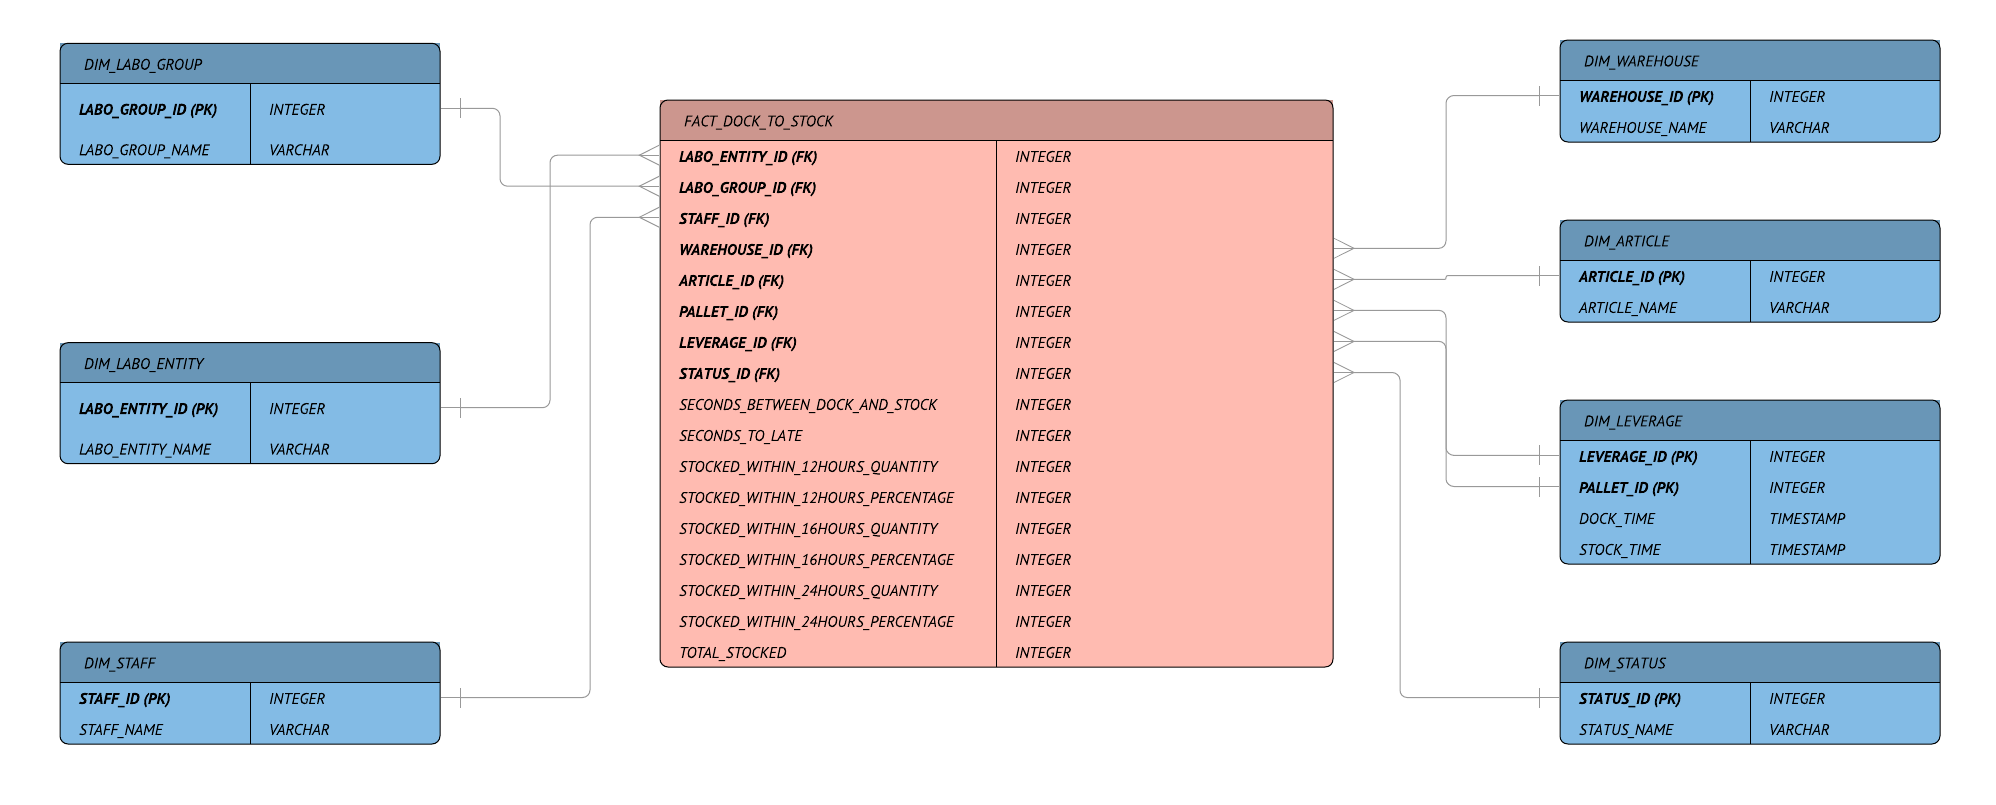
\includegraphics[width=1.0\linewidth]{DimensioneelModel.png}
	\captionof{figure}{\color{HoGentAccent5} Voorstelling van een dimensioneel model (gemaakt via Lucidchart.com).}
	\label{fig:dmdm}
\end{center}\vspace{1cm}

In figuur \ref{fig:dmdm}  worden de dimensions voorgesteld als de blauwe entiteiten. Deze bevatten de beschrijvende data die iets meer vertellen over de ''facts''. De business key wordt gebruikt als attribuut die de relatie legt naar de facts-table (die wordt voorgesteld in het rood). In dit model worden geen gegevens opgeslagen die meer vertellen over de oorsprong van de data, tevens wordt de historiek van de data niet bijgehouden.

\color{HoGentAccent1} 
\subsection*{Data Vault}
\color{black}
Data Vault 2.0 is een modelleertechniek die ontworpen is door Daniel Linstedt. Het model zorgt ervoor dat dimensies gemakkelijk uitgebreid kunnen worden en dat databronnen toevoegen vlot moet gaan. Linstedt is van mening dat business requirements vaak veranderen, dus moet het model waarin de data warehouse ontworpen is ook flexibel zijn(D. Linstedt \& Olschimke, 2016).
\begin{center}\vspace{1cm}
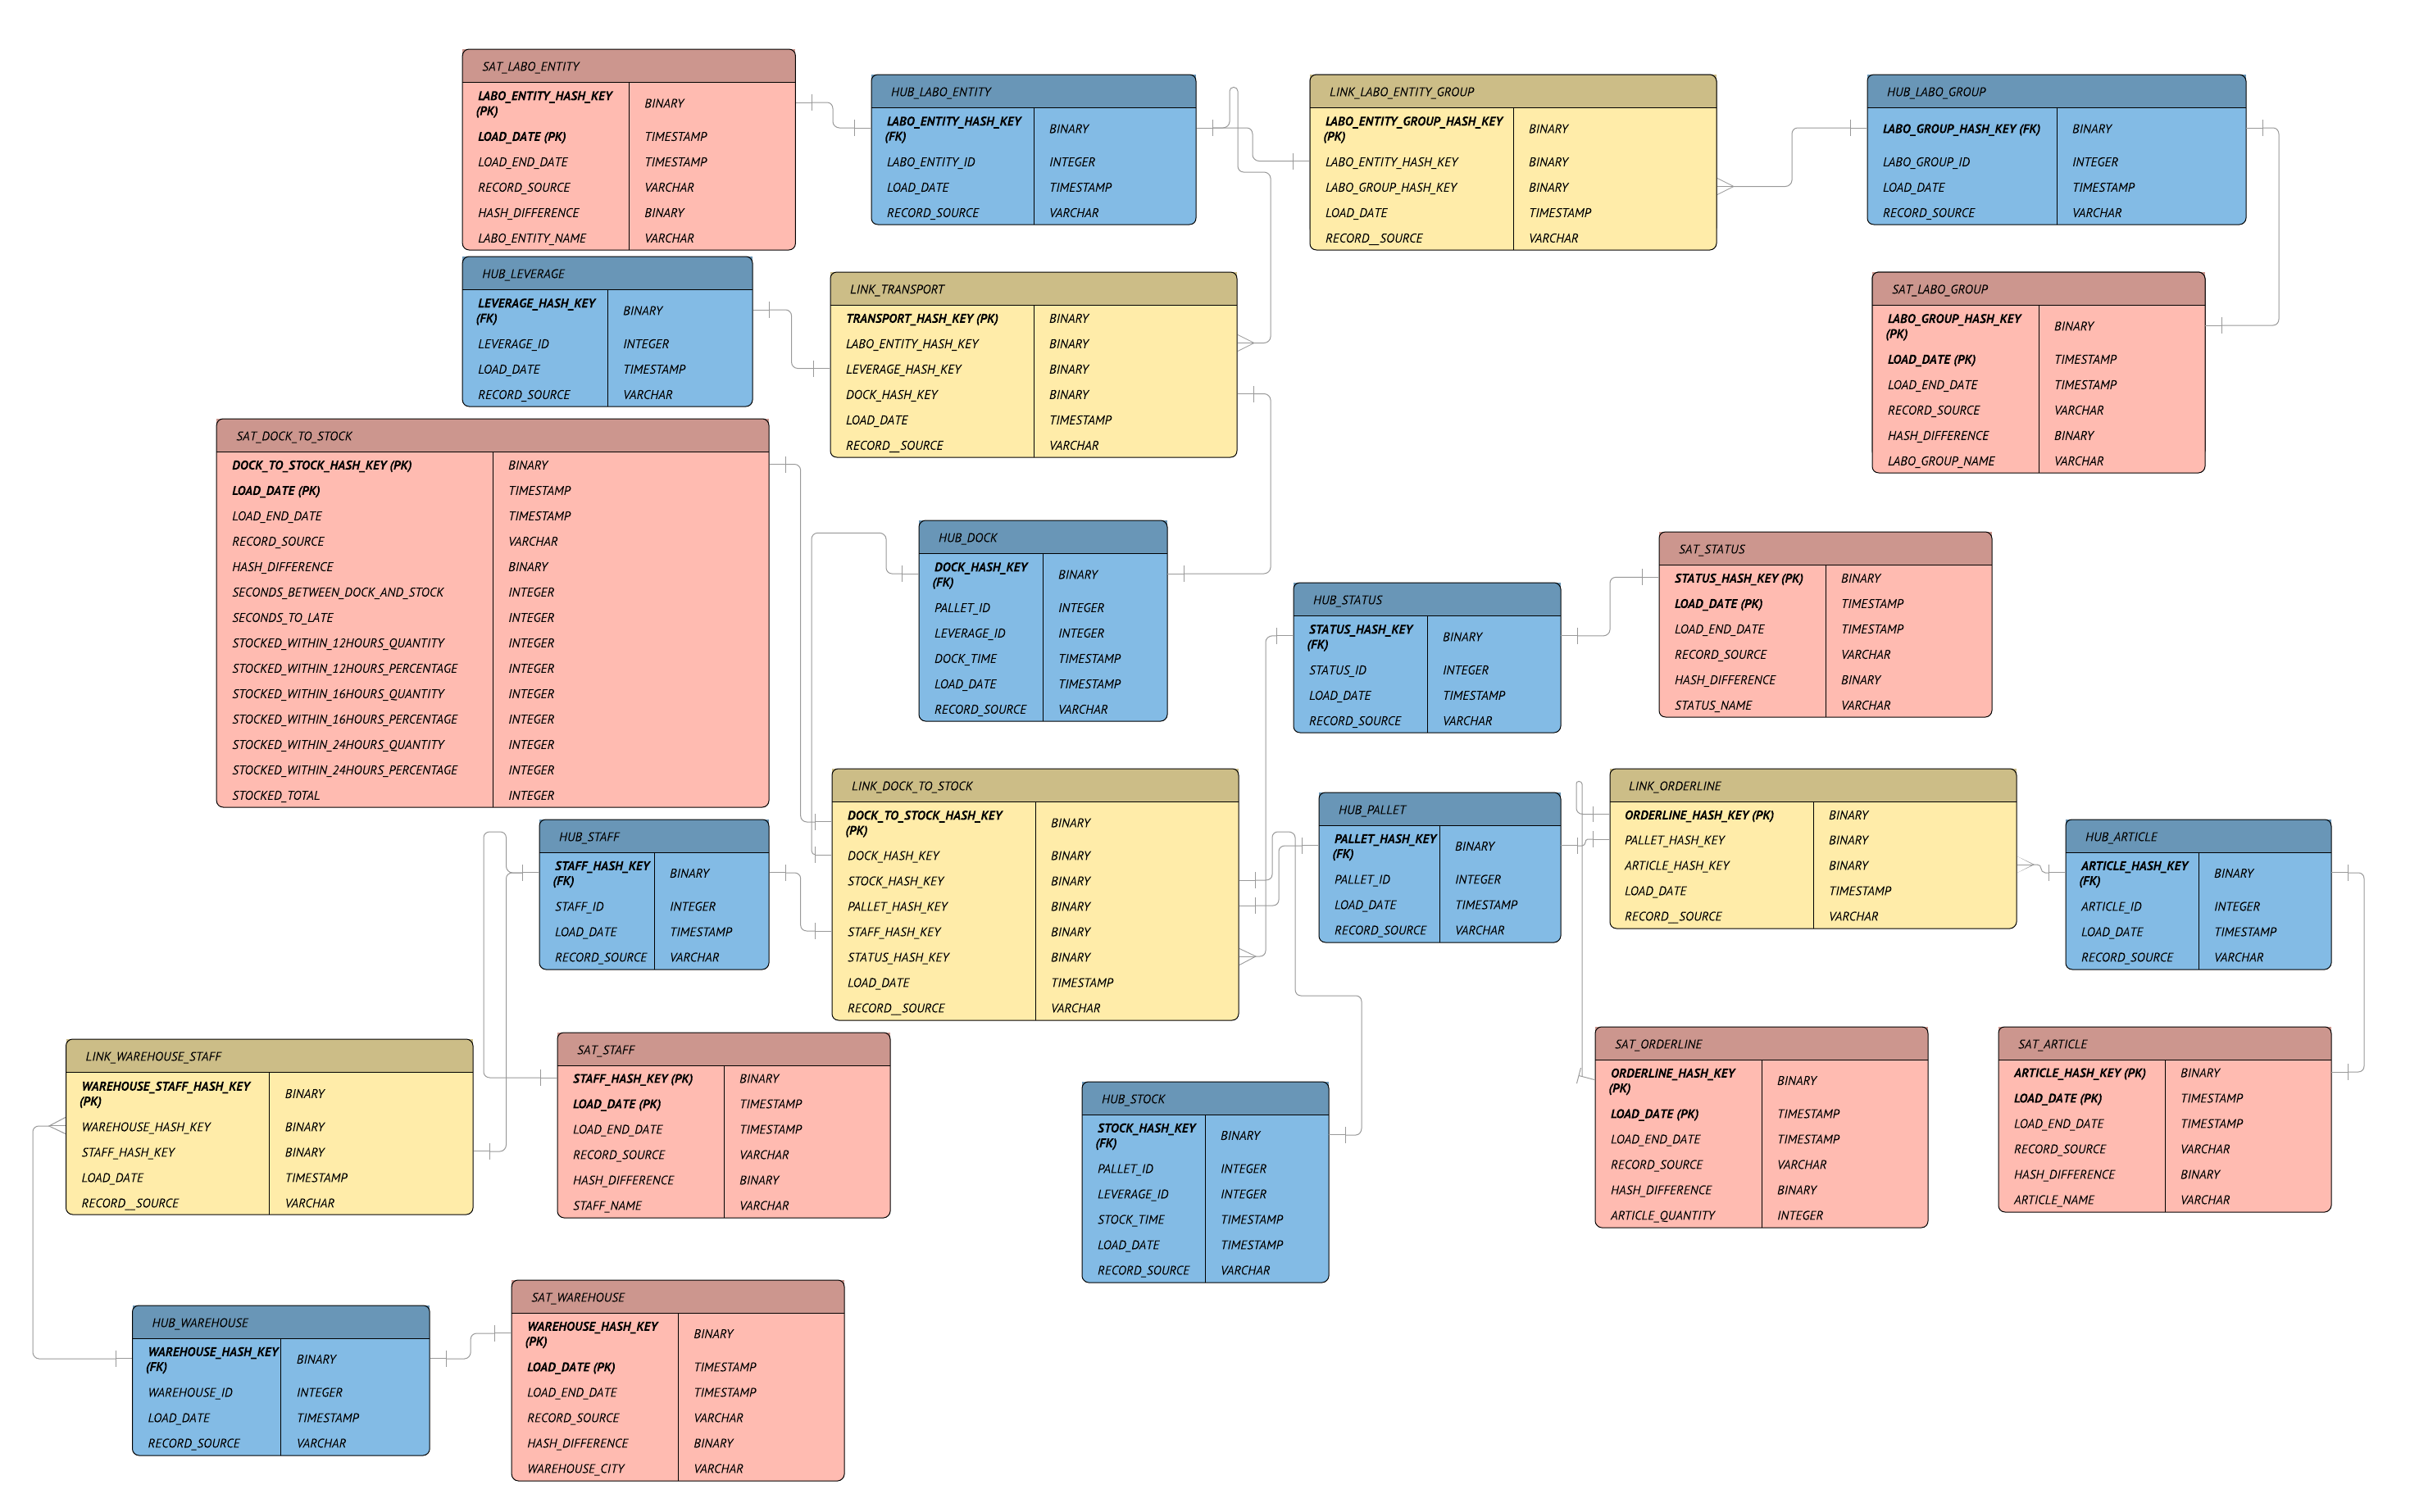
\includegraphics[width=1.0\linewidth]{DataVaultModel.png}
\captionof{figure}{\color{HoGentAccent5} Voorstelling van een Data Vault 2.0 model (gemaakt via Lucidchart.com).}
\label{fig:dvm}
\end{center}\vspace{1cm}
Het model in figuur \ref{fig:dvm} is opgebouwd uit drie soorten tabellen: de rode entiteiten worden voorgesteld als sattelites, de blauwe entiteiten als hubs en de gele entiteiten vormen de links tussen de verschillende hubs. In de SAT\_DOCK\_TO\_STOCK worden de berekeningen opgeslagen die nodig zijn voor het berekenen van de KPI. Hash keys worden gebruikt als primary en foreign keys in dit model en worden opgeslagen onder het type ''binary''.

%------------------------------------------------
\color{HoGentAccent1} 
\section*{Vergelijkende onderzoek}
\color{black}
In deze bachelorproef wordt Data Vault 2.0 vergeleken met het dimensioneel model. In dit vergelijkend onderzoek wordt voornamelijk gefocust op deze 5 pijlers:

\begin{itemize}
	\item \textbf{Performantie:} is er een significant verschil in het uitvoeren van leesopdrachten?
	\item \textbf{Complexiteit:} zijn beide modellen makkelijk interpreteerbaar door IT \& business?
	\item \textbf{Flexibiliteit:} hoe flexibel zijn beide modellen wanneer een business requirement gewijzigd wordt?
	\item \textbf{Schaalbaarheid:} hoe gaan beide modellen overweg met het inladen van enorme hoeveelheid data?
	\item \textbf{Audit:} is er metadata beschikbaar over de werkelijke data? Kunnen problemen makkelijk opgespoord worden?
\end{itemize} 


\color{HoGentAccent1} 
\section*{Conclusies}
\color{black}
Het onderzoek wijst uit dat het dimensioneel model een betere keuze was voor het modelleren van de data voor DHL Pharma Logistics. Dit is bovendien ook het resultaat dat ik verwacht had.

Het dimensioneel model voert sneller leesresultaten uit in vergelijking met het Data Vault, dit omdat het Data Vault model meer relaties heeft. Hierdoor zullen veel meer joins moeten gebeuren wanneer alle data moet opgehaald worden. 

Bij de Data Vault methodologie wordt er meer informatie (Hash keys, informatie over extractie, ..) en tabellen opgeslagen in een databank. Dit zorgt ervoor dat de volumes van data enorm stijgen. Bijgevolg zal er dus een hogere kostprijs zijn om deze data te stockeren. Aangezien dit geen requirement is voor DHL Pharma Logistics, zou dit leiden naar een onnodige meerkost voor dit project.

De KPI's waarvoor een model moet opgesteld worden zijn gestandaardiseerd, en dienen niet flexibel te zijn. Indien de berekening voor de KPI's zouden gewijzigd worden, hoeven enkel sommige parameters uit het ETL-proces aangepast te worden en niet het datamodel zelf.
%----------------------------------------------------------------------------------------
%	FORTHCOMING RESEARCH
%----------------------------------------------------------------------------------------

\color{HoGentAccent1} 
\section*{Toekomstig onderzoek}
\color{black}

Het onderzoek wijst uit dat Data Vault 2.0 een voordeel heeft bij het inladen van data ten opzichte van het dimensioneel model door gebruik te maken van hash keys en doordat tabellen in een Data Vault 2.0 niet afhankelijk zijn van elkaar, kunnen deze allemaal tegelijk ingeladen worden. Naar de toekomst toe kan er onderzocht worden of Data Vault 2.0 een juiste keuze kan zijn bij het opstellen van big data modellen aangezien het toevoegen van enorme volumes data snel en efficiënt kan gebeuren.


%----------------------------------------------------------------------------------------

\end{multicols}
\end{document}